\documentclass[a4paper]{article}

%% Language and font encodings
\usepackage[french]{babel}
\usepackage[utf8x]{inputenc}
\usepackage[T1]{fontenc}

%% Sets page size and margins
\usepackage[a4paper,top=3cm,bottom=2cm,left=3cm,right=3cm,marginparwidth=1.75cm]{geometry}

%% Useful packages
\usepackage{amsmath,amsfonts,amssymb,amsthm,epsfig,epstopdf,titling,url,array}
\usepackage{graphicx}
\usepackage[colorinlistoftodos]{todonotes}
\usepackage[colorlinks=true, allcolors=blue]{hyperref}
\theoremstyle{plain}
\newtheorem{thm}{Théoreme}[section]
\newtheorem{lem}[thm]{Lemme}
\newtheorem{prop}[thm]{Proposition}
\newtheorem*{cor}{Corollary}
\theoremstyle{definition}
\newtheorem{nota}{Notation}[section]
\newtheorem{defn}{Définition}[section]
\newtheorem{conj}{Conjecture}[section]
\newtheorem{exmp}{Exemple}[section]
\theoremstyle{proof}
\newtheorem{dem}{Démonstration}
\theoremstyle{remark}
\newtheorem*{rem}{Remark}
\newtheorem*{note}{Note}

\usepackage{cellspace}
\usepackage{diagbox}

\begin{document}
\begin{titlepage}
  \begin{sffamily}
	\begin{center}
	
		\textsc{\Large Rapport de stage de recherche de mathématiques}\\
		\vspace{9.5cm}
		{ \huge  Les frises de Coxeter \\[0.4cm] }
		
		\vspace{10cm}
		% Author and supervisor
		\begin{minipage}{0.4\textwidth}
			\begin{flushleft} \large
				\textsc{Bétend Marie}\\
			\end{flushleft}
		\end{minipage}
		\begin{minipage}{0.4\textwidth}
			\begin{flushright} \large
				\textsc{Superviseur : M.Bernhard Keller}
			\end{flushright}
		\end{minipage}
		
		\vfill
		
		% Bottom of the page
		{\large 	Mai-Juin 2018}
		
	\end{center}
\end{sffamily}
\end{titlepage}
\tableofcontents
\newpage
\part{Définition}
\section{Exemples}
Voici une frise qui respecte la règle suivante :
pour tout losange \begin{tabular}{ccc}
&b&\\a&&x\\&c& 
\end{tabular}
, $x=\frac{1+bc}{a}$.
\begin{center}
\begin{tabular}{ccccccccccccccccc}
...&0&&0&&0&&0&&0&&0&&0&&0&...\\
1&&1&&1&&1&&1&&1&&1&&1&&1\\
...&2&&1&&4&&1&&2&&2&&2&&1&...\\
3&&1&&3&&3&&1&&3&&3&&1&&3\\
...&1&&2&&2&&2&&1&&4&&1&&2&...\\
1&&1&&1&&1&&1&&1&&1&&1&&1\\
\end{tabular}
\end{center}
On peut remarquer deux choses :
\begin{itemize}
\item Tous les nombres sont des entiers
\item La frise est périodique
\end{itemize}
Regardons une autre frise qui respecte la règle énoncée ci-dessus.
\begin{center}
\begin{tabular}{ccccccccccccccccc}
...&0&&0&&0&&0&&0&&0&&0&&0&...\\
1&&1&&1&&1&&1&&1&&1&&1&&1\\
...&1&&3&&2&&1&&3&&2&&1&&3&...\\
1&&2&&5&&1&&2&&5&&1&&2&&5\\
...&1&&3&&2&&1&&3&&2&&1&&3&...\\
1&&1&&1&&1&&1&&1&&1&&1&&1\\
\end{tabular}
\end{center}
On s'aperçoit que les remarques faites pour la frise précédente sont encore valables. On est alors en droit de se demander si c'est toujours le cas.
\section{Premières définitions}
Commençons tout d'abord par définir formellement ce qu'est une frise.
On peut trouver la définition suivante :

\begin{defn}
Une \textbf{frise}\ est une bande continue et ordonnée sur laquelle un motif se répète de façon régulière et infinie. 
\end{defn}

Mais cette définition est vague, et nous évoque plus facilement des motifs géométriques, commme les frises ci dessous, que des arrangements de nombres.
\\
\begin{center}
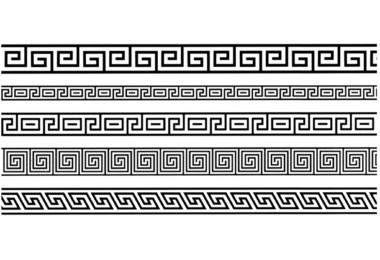
\includegraphics{frise.jpg}
\end{center}
Essayons de définir plus clairement les frises qui nous intéressent dans ce rapport.
\begin{defn}
Une \textbf{frise}\ est une bande infinie, constituée de nombres, arrangés en quinconce, de manière à ce que pour chaque losange 
\begin{tabular}{ccc}
&b&\\a&&c\\&c&
\end{tabular}
on ait $ad-bc=1$.\\
La première rangée est constituée uniquement de 0, tandis que la deuxième et la dernière rangées contiennent uniquement des 1.
Toutes les rangées exceptée la première doivent être composées de nombres réels non nuls.
\end{defn}
On remarque que $d=\frac{1+bc}{a} \Leftrightarrow ad-bc=1$ 
\begin{defn}
On dira que le nombre de rangées d'une frise est son \textbf{ordre}\ et que le nombre de rangées non constituées uniquement de 0 ou de 1 est la \textbf{largeur} de la frise.
\end{defn}
\begin{nota}
On notera \textbf{n}\ l'ordre d'une frise et \textbf{m}\ sa largeur. 
\end{nota}
\begin{exmp}
Sur la première frise que l'on a vu on a $n=6$ et $m=3$.
\begin{center}
\begin{tabular}{ccccccccccccccccc}
...&0&&0&&0&&0&&0&&0&&0&&0&...\\
1&&1&&1&&1&&1&&1&&1&&1&&1\\
...&2&&1&&4&&1&&2&&2&&2&&1&...\\
3&&1&&3&&3&&1&&3&&3&&1&&3\\
...&1&&2&&2&&2&&1&&4&&1&&2&...\\
1&&1&&1&&1&&1&&1&&1&&1&&1\\
\end{tabular}
\end{center}
\end{exmp}

\begin{exmp}
Ici on remarque que la règle n'est pas respectée car $1\times1-1\times1=0$, donc la bande de nombres ci dessous n'est pas une frise au sens où on l'a définit.
\begin{center}
\begin{tabular}{ccccccccccccccccc}
...&0&&0&&0&&0&&0&&0&&0&&0&...\\
1&&1&&1&&1&&1&&1&&1&&1&&1\\
...&1&&1&&1&&1&&1&&1&&1&&1&...\\
1&&1&&1&&1&&1&&1&&1&&1&&1\\
...&1&&1&&1&&1&&1&&1&&1&&1&...\\
1&&1&&1&&1&&1&&1&&1&&1&&1\\
\end{tabular}
\end{center}
En revanche la bande ci dessous est bien une frise.
\begin{center}
\begin{tabular}{ccccccccccccccccc}
...&0&&0&&0&&0&&0&&0&&0&&0&...\\
1&&1&&1&&1&&1&&1&&1&&1&&1\\
...&2&&1&&2&&1&&2&&1&&2&&1&...\\
1&&1&&1&&1&&1&&1&&1&&1&&1\\
\end{tabular}
\end{center}
\end{exmp}

\section{Premiers résultats}
On veut pouvoir étudier les frises. Pour ce faire on décide de noter les élements d'une frise comme des couples d'entiers (r,s). C'est ce qu'on appelle un \textbf{réseau}\ . Avec cette notation on peut retrouver la "position" d'un élément dans une frise donnée.
\\
A une frise d'ordre n correspondra les couples suivants:

\begin{center}
\begin{tabular}{ccccccccccccccccc}
(0;0)&&(1,1)&&(2,2)&&(3,3)&&(4,4)\\
...&(0,1)&&(1,2)&&(2,3)&&(3,4)&&...\\
(-1,1)&&(0,2)&&(1,3)&&(2,4)&&(3,5)\\
...&(-1,2)&&(0,3)&&(1,4)&&(2,5)&&...\\
$\ddots$&&$\ddots$&&$\ddots$&&$\ddots$&&$\ddots$\\
(-s,s)&&(-s+1,s+1)&&(-s+2,s+2)&&(-s+3,s+3)&&(-s+4,s+4)&...\\
\end{tabular}
\end{center}
\begin{nota}
On note \textbf{$f_s$}\ le couple (-1,s) et \textbf{$g_s$}\ le couple (0,s) (correspondant aux deux premières diagonales)
\\
On nomme \textbf{$a_s$}\ l'élément (s-1,s+1) (ce qui correspond aux éléments de la 3ème ligne)
\end{nota}

En réécrivant la définition d'une frise avec la notation en réseau nous avons les propositions suivantes :
\begin{prop}
$\forall r,s \in \mathbb{Z}$ et $r<s<r+n, (r,s)>0$ : $(r-1)(r,s+1)-(r,s)(r-1,s+1)=1$.
\end{prop}

\begin{prop}
Pour $ -1<r<n-1, f_rg_{r+1}-f_{r+1}g_{r}=1$.
\end{prop}

De plus, si on ajoute une ligne de -1 au dessus de la première ligne ou en dessous de la dernière ligne, on ne perd pas en généralités, on a donc la proposition suivante:
\begin{prop}
$\forall r \in \mathbb{R} : $
\begin{itemize}
\item $(r,r)=0$
\item $(r,r+n)=0$
\item $(r,r+1)=1$
\item $(r+1,r+n)=1$
\item $(r,r-1)=-1$
\item $(r-1,r+n)=-1$
\end{itemize}
\end{prop}

\begin{prop}
Pour toute frise, $n=m+3$.
Autrement dit, seules les première,deuxième et dernière rangées sont constituées uniquement de 1 ou de 0. 
\end{prop}

\begin{dem}
On voit que si $m=0$, $n=3$.
Si $m>0$ on peut prendre une ligne qui n'est ni la première, ni la deuxième, ni la dernière. Par définition, cette ligne ne peut pas être composée de 0. Supposons qu'elle soit composée uniquement de 1. Alors on un motif \begin{tabular}{ccc}
&b&\\1&&1\\&c&
\end{tabular} dans la frise. On a $1-b\times c=1 \Leftrightarrow bc=0$. Or, c ne peut pas valoir 0 car il n'y a des 0 que sur la première ligne. Alors b vaut 0 et donc la ligne que nous avons prise ne peut être que la deuxième et il y a une contradiction avec le choix de la ligne.
Finalement, les seules rangées constituées uniquement de 1 sont la deuxième et la dernière.
\end{dem}

\begin{thm}
$\forall r,s \in \mathbb{Z}$ tels que $0\le r\le s\le n-1$ on a $(r,s)=f_rg_s-f_sg_r$.
\end{thm}
\begin{dem}
On va procéder par récurrence.
Si $r=0$, on a $(r,f)=g_s=1\times g_s -0$ et $g_0=0$,$f_0=1$.
Supposons la propriété est vraie pour ($0\le r'\le r$ et $r'\le s'\le r'+n$) et($r'=r+1$ et $r'\le s'\le s$).

Si $r=s$, alors $(r+1,s+1)=0=f_{r+1}g_{s+1}-f_{s+1}g_{r+1}$. 

Sinon $(r,s)=f_rg_s-f_sg_r \neq 0$.

En appliquant la loi unimodulaire, on a $(r,s)(r+1,s+1)-(r+1,s)(r,s+1)=1$, d'où $(r+1,s+1)=\frac{1+(r+1,s)(r,s+1)}{(r,s)}=\frac{1+(f_{r+1}g{s}-f_sg_{r+1})(f_rg_{s+1}-f_{s+1}g_r}{f_rg_s-f_sg_r}$

$(r+1,s+1)=\frac{1+f_rf_{r+1}g_sg_{s+1}-f_{r+1}f_{s+1}g_sg_r-f_sf_rg_{r+1}g_{s+1}+f_sf_{s+1}g_rg_{r+1}}{f_rg_s-f_sg_r}$

Or $f_rg_{r+1}-f_{r+1}g_r=1$, d'où 

$(r+1,s+1)=\frac{1+f_rf_{r+1}g_sg_{s+1}+f_sf_{s+1}g_rg_{r+1}-f_sg_{s+1}(1+f_{r+1}g_r)-f_{s+1}g_s(f_rg_{r+1}-1)}{f_rg_s-f_sg_r}$

$(r+1,s+1)=\frac{1-f_sg_{s+1}-f_{s+1}g_s}{f_rg_s-f_sg_r}+f_{r+1}g_{s+1}-f_{s+1}g_{r+1}$

$(r+1,s+1)=f_{r+1}g_{s+1}-f_{s+1}g_{r+1}$

Par récurrence la propriété est prouvée.
\end{dem}
\part{Propriétés}
\section{Périodicité d'une frise}
On se souvient qu'on avait remarqué que les frises semblaient se répeter sur des exemples, voyons si nous pouvons le démontrer.

\begin{lem}
$\forall r,s,t,u \in \mathbb{Z}, (r,s)(t,u)+(r,t)(u,s)+(r,u)(s,t)=0$
\end{lem}

\begin{dem}
En développant on a : 
\begin{itemize}
\item $(r,s)(t,u)=(f_rg_s-f_sg_r)(f_tg_u-f_ug_t)=f_rf_tg_sg_u-f_rf_ug_sg_t-f_sf_tg_rg_u+f_sf_ug_rg_t$
\item $(r,t)(u,s)=(f_rg_t-f_tg_r)(f_ug_s-f_sg_u)=f_rf_ug_tg_s-f_rf_sg_tg_u-f_tf_ug_rg_s+f_tf_sg_ug_r$
\item $(r,u)(s,t)=(f_rg_u-f_ug_r)(f_sg_t-f_tg_s)=f_rf_sg_ug_t-f_rf_tg_ug_s-f_uf_sg_rg_t+f_uf_tg_rg_s$
\end{itemize}
Finalement, $(r,s)(t,u)+(r,t)(u,s)+(r,u)(s,t)=f_rf_tg_sg_u-f_rf_ug_sg_t-f_sf_tg_rg_u+f_sf_ug_rg_t+f_rf_ug_tg_s-f_rf_sg_tg_u-f_tf_ug_rg_s+f_tf_sg_ug_r+f_rf_sg_ug_t-f_rf_tg_ug_s-f_uf_sg_rg_t+f_uf_tg_rg_s=0$
\end{dem}

\begin{lem}
$\forall r,s \in \mathbb{Z}, (r,s)=-(s,r)$
\end{lem}
\begin{dem}
De nouveau, en développant, on a $(r,s)=f_rg_s-f_sg_r=-(f_sg_r-g_rg_s)=-(s,r)$
\end{dem}

\begin{thm}
Pour une frise d'orde n, $\forall r,s \in \mathbb{Z}, (r,s)=(s,r+n)=(s+n,r)=(r+n,s+n)$.

En particulier, $\forall s \in \mathbb{Z}, f_{s+n}=f_s$ et $a_{s+n}=a_s$ 
\end{thm}
\begin{dem}
On sait que $\forall r,s,t,u \in \mathbb{Z}, (r,s)(t,u)+(r,t)(u,s)+(r,u)(s,t)=0$, don en posant $t=r+1$ et $u=r+n$, on a $(r,s)(r+1,r+n)+(r,r+1)(r+n,s)+(r,r+n)(s,r+1)=0$.

Or $(r+1,r+n)=1$, $(r,r+1)=1$ et $(r,r+n)=0$ donc 

$(r,s)+(r+n,s)=0 \Leftrightarrow (r,s)=-(r+n,s) \Leftrightarrow (r,s)=(s,r+n)$ d'après le lemme 2.

En posant $r'=s$ et $s'=r+n$ on a $(s,r+n)=(r',s')=(s',r'+n)=(r+n,s+n)=(r,s)$ donc $(s,r+n)=(r,s)$.

De plus, $(s+n,r)=(r,s) \Leftrightarrow (s,r)=(r,s+n)$
\end{dem}

Finalement, nous avons vu que (r,s)=(r+n,s+n), donc une frise d'ordre n est périodique de période n. De plus comme (r,s)=(s,r+n) on sait que le motif est triangulaire, et qu'il engendre toute la frise. On appelle ce triangle, \textbf{triangle fondamental}. On obtient la frise en répetant ce triangle et son symétrique par rapport à l'horizontal.

\begin{exmp}
\begin{center}
\begin{tabular}{ccccccccccccccccc}
...&0&&0& \diagbox[dir=SW]{}{} &0&\diagbox{}{}&0&&0&&0&&0&&0&...\\
1&&1&\diagbox[dir=SW]{}{}&1&&1&\diagbox{}{}&1&&1&&1&&1&&1\\
...&2&\diagbox[dir=SW]{}{}&1&&4&&1&\diagbox{}{}&2&&2&&2&&1&\diagbox[dir=SW]{}{}\\
3&\diagbox[dir=SW]{}{}&1&&3&&3&&1&\diagbox{}{}&3&&3&&1&\diagbox[dir=SW]{}{}&3\\
\diagbox[dir=SW]{}{}&1&&2&&2&&2&&1&\diagbox{}{}&4&&1&\diagbox[dir=SW]{}{}&2&...\\
1&&1&&1&&1&&1&&1&\diagbox{}{}&1&\diagbox[dir=SW]{}{}&1&&1\\
\end{tabular}
\end{center}
\end{exmp}
\section{Quelques propriétés}
\begin{prop}
$\forall r,s \in \mathbb{Z}, (r,s+1)=a_s(r,s)-(r,s-1)$.

En particulier, $\forall s \in \mathbb{Z}, f_{s+1}+f_{s-1}=a_sf_s$.
\end{prop}

\begin{dem}
D'après le lemme 1, on a $(r,s)(s-1,s+1)+(s,s+1)(s-1,r)+(s+1,r)(s-1,s)=0$.
Autrement dit, $a_s(r,s)-(r,s+1)-(r,s+1)=0$ d'après le lemme 2.
\end{dem}

\begin{prop}
$\forall r, s\in \mathbb{Z}$ tels que $s \ge r+2$, $(r,s)= \begin{vmatrix}
a_{r+1}&1&0&0&...&0\\
1& a_{r+2}&1&0&...&0\\
\vdots&\ddots&\ddots&\ddots&\ddots&\vdots\\
0&...&0&1&a_{s-2}&1\\
0&...&0&0&1&a_{s-1}
\end{vmatrix}$

En particulier, $\forall s \in \mathbb{N}$, $f_{s+1}=\begin{vmatrix}
a_{0}&1&0&0&...&0\\
1& a_{1}&1&0&...&0\\
\vdots&\ddots&\ddots&\ddots&\ddots&\vdots\\
0&...&0&1&a_{s-1}&1\\
0&...&0&0&1&a_{s}
\end{vmatrix}$.
\end{prop}

\begin{dem}
On prend un r $\in \mathbb{Z}$ quelconque, et on procède par réccurence double sur s.

$(r,r+2)=a_{r+1}$

$(r,r+3)=a_{r+2}(r,r+2)-(r,r+1)$

Donc $(r,r+3)=a_{r+2}a_{r+1}-1=\begin{vmatrix}
a_{r+1}&1\\
1&a_{r+2}
\end{vmatrix}$

Supposons maintenant la propriété vraie au rang s et s+1, avec $s\ge r+2$.

On commence par développer par rapport à la dernière ligne :

$\begin{vmatrix}
a_{r+1}&1&0&0&...&0\\
1& a_{r+2}&1&0&...&0\\
\vdots&\ddots&\ddots&\ddots&\ddots&\vdots\\
0&...&0&1&a_{s}&1\\
0&...&0&0&1&a_{s+1}
\end{vmatrix}
= a_{s+1}(r,s+1)- \begin{vmatrix}
a_{r+1}&1&0&0&...&0\\
1& a_{r+2}&1&0&...&0\\
\vdots&\ddots&\ddots&\ddots&\ddots&\vdots\\
0&...&0&1&a_{s-1}&1\\
0&...&0&0&1&1
\end{vmatrix}$

Puis on développe par rapport à la dernière colonne :

$a_{s+1}(r,s+1)- \begin{vmatrix}
a_{r+1}&1&0&0&...&0\\
1& a_{r+2}&1&0&...&0\\
\vdots&\ddots&\ddots&\ddots&\ddots&\vdots\\
0&...&0&1&a_{s-1}&1\\
0&...&0&0&1&1
\end{vmatrix}=
a_{s+1}(r,s+1)-(r,s)=(r,s+2)$

Par récurrence la propriété est prouvée.
En évaluant en r=-1, on obtient la propriété pour les $f_s$.
\end{dem}
\begin{defn}
Une frise \textbf{entière}\ est une frise dont tous les coefficients sont des entiers.
\end{defn}

\begin{exmp}
\begin{center}
\begin{tabular}{ccccccccccccccccc}
...&0&&0&&0&&0&&0&&0&&0&&0&...\\
1&&1&&1&&1&&1&&1&&1&&1&&1\\
...&$\sqrt{2}$&&$\sqrt{2}$&&$\sqrt{2}$&&$\sqrt{2}$&&$\sqrt{2}$&&$\sqrt{2}$&&$\sqrt{2}$&&$\sqrt{2}$&...\\
1&&1&&1&&1&&1&&1&&1&&1&&1\\
\end{tabular}
\end{center}
Ce n'est pas une frise entière.
\end{exmp}

\begin{prop}
Soit $\mathcal{F}$ une frise d'orde n. Il y a équivalence entre ces trois propriétés :
\begin{enumerate}
\item $\mathcal{F}$ est entière
\item $\forall s \in \mathbb{Z}$ tel que $-1<s<n-2$, $f_s\in \mathbb{N}$ et $f_s|f_{s-1}+f_{s+1}$
\item $\forall s\in \mathbb{Z}$, $a_s \in \mathbb{N}$
\end{enumerate}

De plus si $\mathcal{F}$ est entière, $\forall r, s$ tels que $r<s<r+n-1$, $(r,s)|(r,s-1)+(r,s+1)$.
\end{prop}

\begin{dem}
\begin{enumerate}
\item $\forall r, s \in \mathbb{Z}$ tels que $r<s<r+n-1$, $(r,s)\in \mathbb{N}$ et$(r,s)|(r,s-1)+(r,s+1)$
\item$\forall s \in \mathbb{Z}$ tel que $-1<s<n-2$, $f_s\in \mathbb{N}$ et $f_s|f_{s-1}+f_{s+1}$
\item $\forall s\in \mathbb{Z}$, $a_s \in \mathbb{N}$
\end{enumerate}

On voit clairement que $1 \Rightarrow 2$. 

$2 \Rightarrow 3$ se déduit de la relation $f_sa_s=f_{s-1}+f_{s+1}$.

$3 \Rightarrow$ :

Si $s=r+1,(r,s)=1 \in \mathbb{N}$.

Sinon, si $s \ge r+2, (r,s)=\begin{vmatrix}
a_{r+1}&1&0&0&...&0\\
1& a_{r+2}&1&0&...&0\\
\vdots&\ddots&\ddots&\ddots&\ddots&\vdots\\
0&...&0&1&a_{s-2}&1\\
0&...&0&0&1&a_{s-1}
\end{vmatrix}$, donc (r,s) $\in \mathbb{N}$ car tous les $a_i \in \mathbb{N}$ et le déterminant est un polynôme des coefficients de la matrice. Comme on est dans une frise, (r,s) $\neq$0 et on a donc bien $\forall r,s \in \mathbb{Z}$ tels que $r<s<r+n-1$, $(r,s-1)+(r,s+1)\in \mathbb{N*}$.

Or $a_s(r,s)=(r,s+1)+(r,s-1)$, donc $(r,s)|(r,s-1)+(r,s+1)$.
\end{dem}
\part{Bijection}
\section{Triangulation de polygones convexes}
\begin{defn}
Une \textbf{triangulation}\ d'un polygone $\mathcal{P}$ est une partition de $\mathcal{P}$ en un ensemble de triangles qui ne se superposent pas et dont l'union forme $\mathcal{P}$. Les sommets des triangles doivent être les sommets de $\mathcal{P}$.
\end{defn}

On peut voir sur la figure ci dessous différentes triangulations pour plusieurs polygones.
\begin{center}
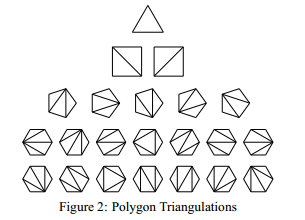
\includegraphics[]{triangulation.jpg}
\end{center}

Sur cette figure on remarque que le nombre de triangle est toujours le même, est-ce toujours le cas ?

\begin{prop}
Un polygone triangulé à n sommets possède n-2 triangles et n-3 diagonales.
\end{prop}

\begin{dem}
Procédons par récurrence : si n=3, nous avons un triangles qui possède bien 1 triangle et 0 diagonales.

Supposons que la propriété soit vraie au rang n, et $\forall k\le n$, et vérifions qu'elle est toujours vraie au rang n+1.

Prenons donc un polygone triangulé à n+1 sommets. On choisit une diagonale au hasard qui sépare notre polygone en deux sous polygones de k et n-k+2 sommets. D'après notre hypothèse de récurrence, ces sous polygones contiennent respectivement k-2 et n-k triangles, et k-3 et n-k-1 diagonales.

Donc notre polygone possède $(k-2)+(n-k)=n-2$ triangles et $(k-3)+(n-k-1)+1=n-3$ diagonales.
Par récurrence, notre hypothèse est prouvée.
\end{dem}

On peut également se demander quel est le nombre de triangulation possible pour un polygone donné.
Pour répondre à cette question, on va admettre le théorème suivant :

\begin{thm}
Soit $n\ge 3$, l'ensemble des n-gones convexes triangulés est en bijection avec l'ensemble des arbres binaires à n-2 noeuds ( c'est à dire n-1 feuilles).
\end{thm}

Sur l'image si dessous, on peut voir qu'a différentes triangulations, on peut associer différents arbres binaires.
\begin{center}
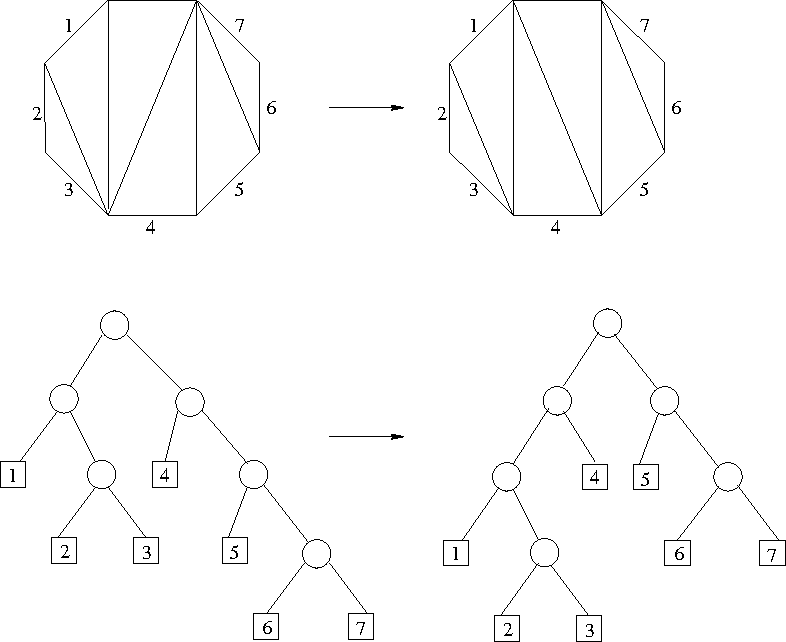
\includegraphics[scale=0.5]{triang-bina.png}
\end{center}

Ce théorème est pratique car il est plutôt facile de compter combien d'arbres binaires à n noeuds possibles existent. Cela nous permet donc de répondre à notre question.

\begin{prop} 
On note $c(n)$ le nombre d'arbres binaires à n feuilles.

$c(n)=\frac{(2n)!}{(n+1)!n!}=\frac{1}{n+1}\binom{2n}{n}$
\end{prop}
La démonstration ne sera pas faite ici non plus car il s'agit d'un calcul un peu fastidieux, mais je vous renvoi vers le rapport de stage sur les frises d'Adrien Laurent pour plus de détails.

Les c(n) sont appelés nombres de Catalan et sont utilisés dans divers problèmes de dénombrement.

Il existe donc $c(n-2)$ triangulations possibles d'un n-gones convexe, c'est à dire $\frac{(2n-4)!}{(n-1)!(n-2)!}$.

\section{Bijection entre triangulations et frises}
On souhaite désormais montrer que l'ensemble des frises d'ordre n et celuis des triangulations de n-gones convexes, sont en bijection. Pour cela nous allons utiliser les deux lemmes suivants :

\begin{lem}
Dans une frise entière $\mathcal{F}$, il y a au moins un des éléments de $(a_0,a_1,a_2,...,a_n)$ égal à 1.
\end{lem}

\begin{defn}
On appelle $(a_0,a_1,a_2,...,a_n)$ le \textbf{cycle de quiddité}\ d'une frise $\mathcal{F}$ d'orde n.
\end{defn}

\begin{dem}
Utilisons un raisonnement pas l'absurde.

On sait que $\forall s \in \mathbb{N}$ tel que $s<n-1$, on a $a_sf_s=f_{s+1}+f_{s-1}$. Si tous les $a_s$ sont supérieurs ou égaux à 2, on peut écrire $f_{s+1}\ge 2f_s-f_{s-1}$.
Or $f_{s+1}-f_s\ge f_s-f_{s-1}\ge ... \ge f_0-f_1=1$, d'où $f_s\ge s+1$.

On a donc  $f_{n-2}=1\ge n-1$ ce qui est absurde, donc finalement, il y a au moins un des $a_s$ inférieur à 2, et comme il ne peut pas être nul, il vaut 1.
\end{dem}

\begin{lem}
Si on connait un  cycle de quiddité de la forme (... t u v w ...), qui engendre une frise entière $\mathcal{F}$ d'orde n (n$_ge$4), alors le cycle (... t u+1 1 v+1 w ...) engendre une frise entière $\mathcal{F'}$ d'ordre n+1.

Réciproquement, si on connait une frise entière $\mathcal{F'}$ d'orde n (n$\ge$5) engendré par un cycle de quiddité de la forme (... t' u' 1 v' w' ...), le cycle (... t' u'-1 v'-1 w'...) engendre une frise entière $\mathcal{F}$ d'ordre n-1.
\end{lem}

\begin{dem}
Soit $n \ge 4$ et soit $\mathcal{F}$ une frise entière d'ordre n engendré par un cycle de quiddité de la forme (... t u v w ...). La diagonale des $f_s$ de $\mathcal{F}$ est de la forme ... T U V W ... avec $u=\frac{T+V}{U}$ et $v=\frac{U+W}{V}$. De plus comme $\mathcal{F}$ est entière, $U|T+V$ et $V|U+W$.

Si on glisse un U+V dans la diagonale, on a bien $U+V|U+V$ et U+V$\in \mathbb{N*}$, donc la diagonale ...T U U+V V W ... engendre une frise entière d'ordre n+1.

Le cycle de quiddité associé à cette frise est (... t u' x v' w ...), avec $u'=\frac{T+(U+V)}{U}=u+1$, $v'=\frac{(U+V)+W}{V}=v+1$ et $x=\frac{U+V}{U+V}=1$.

On prouve la réciproque de la même manière.
\end{dem}

\begin{defn}
Soit $P_0P_1...P_{n-1}$ un n-gone gonvexe.

On définit $\phi_{P_0P_1...P_{n-1}}$ pour $n\ge 3$, comme l'application qui à une frise $\mathcal{F} $ associe une triangulation de $P_0P_1...P_{n-1}$, définie par : $\forall s \in \mathbb{N}$ avec $0\le s\le n-1$, $a_s$ correspond au nombre de triangles dont un des sommets est $P_s$.
\end{defn}

\begin{exmp}
Lorsque n=3, il ya une seule frise possible, avec un cycle de quiddité valant (1 1 1).
Un triangle quant à lui admet une seule triangulation, avec un seul triangle lui même, donc chaque sommet est bien le sommet d'un seul triangle.

Lorsque n=4, il y a deux frises possibles, de cycles de quiddité valant (1,2,1,2) et (2,1,2,1).
Un 4-gone quand à lui admet 2 triangulations , comme illustré sur l'image ci dessous.

\begin{center}
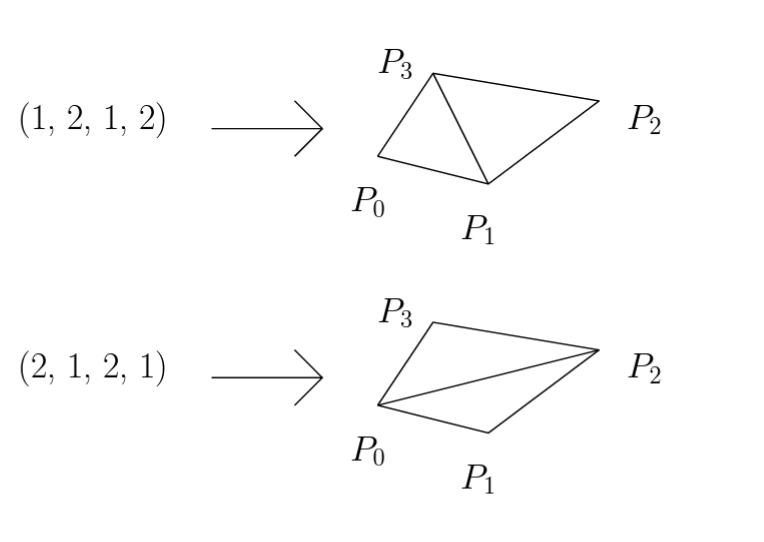
\includegraphics[scale=0.4]{tria.png}
\end{center}
\end{exmp}
\begin{prop}
$\phi_{P_0P_1...P_{n-1}}$ est bien définie pour tout $n\ge 3$ et tout polygone $P_0P_1...P_{n-1}$.
\end{prop}

\begin{dem}
Le cycle de quiddité suffit à définir une frise, donc on peut bel et bien associer une frise à une triangulation.

On procède par récurrence.

On a vu que lorsque n=3 ou n=4 la proposition est vraie.

Supposons maintenant qu'elle soit vraie pour un n$\ge4$.

Soit $P_0P_1...P_{n}$ un n+1-gone et $\mathcal{F}_{n+1}$ une frise entière d'orde n+1.
On veut montrer qu'il existe une seule triangulation de $P_0P_1...P_{n}$ correspondant au cycle de quiddité de $\mathcal{F}_{n+1}$.

Existence :

Quitte à tourner notre polygone, on suppose $a_n=1$ (étant donné qu'il y a au moins un 1 dans le cycle de quiddité). On crée maintenant une frise entière $\mathcal{F}_n$ engendrée par $(a_0-1,a_1,...,a_{n-1}-1)$ (cf lemme 7.2). D'après notre hypothèse de récurrence, $\phi_{P_0P_1...P_{n-1}}$ est définie, et donc $\phi_{P_0P_1...P_{n-1}}(\mathcal{F}_n)$ est une triangulation de $P_0P_1...P_{n-1}$.

On construit alors une triangulation de $P_0P_1...P_{n}$ en ajoutant un triangle (aussi appelé oreille ici), sur le côté $P_0P_{n-1}$. Cette triangulation correspond à la frise $\mathcal{F}_{n+1}$, car il y a bien $(a_0-1)+1$ triangles touchant $P_0$, $(a_{n-1}-1)+1$ triangles touchant $P_{n-1}$, 1=$a_n$ triangle touchant $P_n$ et $a_s$ triangles touchant les autres sommets $P_s$.

L'existence est bien prouvée, montrons maintenant que cette frise est unique.


Unicité:

Comme la triangulation $P_0P_1...P_{n-1}$ est l'unique possible, nous avons une seule possibilité pour rajouter $P_n$: par le triangle $P_0P_{n-1}P_n$. D'où la triangulation $P_0P_1...P_{n}$ est unique.

Finalement, $\phi_{P_0P_1...P_{n-1}}$ est bien définie.
\end{dem}

Maintenant que nous avons tous les éléments nécessaires, prouvons le théorème suivant.

\begin{thm}
L'ensemble des frises entières d'ordre n est en bijection avec l'ensemble des triangulations de n-gones convexes. 
\end{thm}

\begin{dem}
Pour ce théorème nous allons montrer que $\forall$ n$\ge$3, $\forall P_0P_1...P_{n-1}$ polygone convexe, $\phi_{P_0P_1...P_{n-1}}$ est une bijection.



Injectivité:

Prenons deux frises entières $\mathcal{F}$ et $\mathcal{F'}$ d'orde n.Si $\phi_{P_0P_1...P_{n-1}}(\mathcal{F})=\phi_{P_0P_1...P_{n-1}}(\mathcal{F'}$, alors le nombre de triangles touchant $P_0P_1...P_{n-1}$ sont les mêmes, ce qui veut dire que $\mathcal{F}$ et $\mathcal{F'}$ ont le même cycle de quiddité. Or le cycle de quiddité définit entièrement la frise, donc $\mathcal{F}=\mathcal{F'}$.



Surjectivité:
On va de nouveau procéder par récurrence. On sait que pour n=3 et n=4, la surjectivité est avérée.

On suppose que pour n$\ge$4 $\phi_{P_0P_1...P_{n-1}}$ est surjective.

Soit $P_0P_1...P_n$ un n+1-gone convexe. On peut lui associer le cycle $(a_0 ... a_n)$ du nombre de triangle touchant chacun des sommets. On veut montrer que ce cycle engendre une frise.

On commence par remarquer qu'au moins un des $a_i$ vaut 1 car tous polygone triangulé,sauf un triangle, possède au moins 2 oreilles (sommet touchant un seul triangle).

On peut maintenant utiliser le lemme 7.2 et réduire le cycle $(a_0 ... a_n)$ en un cycle de quiddité de longueur n. Or on sait que ce nouveau cycle engendre une frise d'ordre n, donc d'après le lemme 7.2, toujours, notre cycle $(a_0 ... a_n)$ engendre bien une frise entière d'ordre n+1.

Finalement, $\phi_{P_0P_1...P_{n-1}}$ est bien une surjection, et la récurrence est prouvée.

D'où, $\forall$ n$\ge$3, $\forall P_0P_1...P_{n-1}$ polygone convexe, $\phi_{P_0P_1...P_{n-1}}$ est une bijection.

\end{dem}

\part{Pour conclure}
Les frises peuvent à première vue paraitre être des objets abstraits et sans grande utilité, j'étais d'ailleurs étonnée au début que l'on puisse démontrer quoi que ce soit sur des objets d'une grandeur infinie, et j'étais assez dubitative sur le fait d'y comprendre quoi que ce soit.

Finalement, je me suis vite rendue compte que le sujet était plus abordable qu'il n'y paraissait et que je prenais même plaisir à décortiquer les démonstrations des théorèmes pour mieux les comprendre.

En plus de cela j'ai pu me rendre compte que les relations entre les différents objets mathématiques peuvent être cachées de manières insoupçonnables.

Je tiens à remercier Mr Bernhard Keller pour avoir pris le temps de m'initier à ce sujet et d'avoir répondu à mes questions.

Je tiens également à signaler que ce stage s'est entièrement basé sur le rapport de stage sur les frises  d'Adrien Laurent, et que mon rapport n'est qu'une petite réecriture du sien.
\end{document}   